%        File: spectral.tex
%     Created: 日 6月 16 03:00 下午 2019 C
% Last Change: 日 6月 16 03:00 下午 2019 C
%
\documentclass[xcolor={svgnames}]{beamer}
\usetheme[
  numbering=fraction, % curr_page / total_page
  block=fill,         % 为 block 显示方框
  % progressbar=frametitle % add a progressbar at frametitle
  sectionpage=progressbar
]{metropolis}

%% 保留熟悉的数学字体:两种方法
% \usefonttheme[onlymath]{serif}
\renewcommand\mathfamilydefault{\rmdefault}

% include predefined commands
\input ../defs.tex  % some frequently used alias

%% additional alias
\newcommand{\lipnorm}[1]{\lVert #1 \rVert_\mathrm{Lip}}
\newcommand{\snmat}{\bar{W}_{\mathrm{SN}}}

\usepackage[english]{babel}
% \usepackage{enumitem} % 支持自定义 item symbol
\usepackage{tikz}
\usetikzlibrary{tikzmark,positioning,shapes,calc}
\usepackage{mathtools}
\usepackage{fancybox}   %支持文本框
\usepackage{subfig}     %支持subfi
\usepackage{cite}
%\usepackage{biblatex}
%\usepackage[backend=biber,style=numeric-comp,sorting=none]{biblatex}
%\addbibresource{int-ref.bib}

% Removes icon in bibliography
\setbeamertemplate{bibliography item}[text]

% add following for otherwise it will complain
% see https://tex.stackexchange.com/questions/426088/texlive-pretest-2018-beamer-and-subfig-collide
\makeatletter
\let\@@magyar@captionfix\relax
\makeatother
%%%

%=== font customization ===%
%%
%% Note that once use customizing fonts, switch to xelatex
%%
% \usepackage{fontenc}
% \setsansfont{Varela Round}
% % \setsansfont{IM FELL DW Pica}
% \setmonofont{DejaVu Sans Mono}
% \setmathfont{Fira Sans}


%% 目录标数字
\setbeamertemplate{section in toc}[sections numbered]
%% 无序列表用实心点
% \setbeamertemplate{itemize item}{$\bullet$}
% \setbeamertemplate{navigation symnols}{}

%% 设置列表的 item symbol
\setbeamertemplate{itemize item}{\textbullet}
\setbeamertemplate{itemize subitem}{$\blacktriangleright$}
\setbeamertemplate{itemize subsubitem}{$\checkmark$}

%% 定理环境计数
\setbeamertemplate{theorems}[numbered]
% \setbeamertemplate{lemmas}[numbered]

% 定义颜色
\definecolor{alizarin}{rgb}{0.82, 0.1, 0.26} % 红色
\definecolor{DarkFern}{HTML}{407428}         % 绿色
\definecolor{bistre}{rgb}{0.24, 0.17, 0.12}  % 黑色
\definecolor{mygrey}{rgb}{0.52, 0.52, 0.51}  % 灰色
\definecolor{tyorange}{HTML}{ff6600}         % 天依橙
\definecolor{tyblue}{HTML}{0066ff}           % 天依蓝
\colorlet{main}{DarkFern!100!white}          % 第一种设置方法
\colorlet{main}{red!70!black}                % 第二种设置方法
\colorlet{main}{tyblue}
\colorlet{text}{bistre!100!white}

% 不同元素指定不同颜色,fg是本身颜色,bg是背景颜色,!num!改变数值提供渐变色
% \setbeamercolor{title}{fg=main}
% \setbeamercolor{frametitle}{fg=main}
% \setbeamercolor{section in toc}{fg=text}
% \setbeamercolor{normal text}{fg=text}
% \setbeamercolor{block title}{fg=alizarin,bg=mygrey!20!white}
% \setbeamercolor{block body}{fg=black,bg=mygrey!15!white}
% \setbeamercolor{qed symbol}{fg=main} % 证明结束后的框颜色
% \setbeamercolor{math text}{fg=black}

%=== set theme background color to white ===%
%\setbeamercolor{background}{bg=tyblue}
\setbeamercolor{alerted text}{fg=red!50!black}
\setbeamercolor{normal text}{fg=black!85!}
\setbeamercolor{example text}{fg=black!50!cyan}
%\setbeamercolor{frametitle}{bg=tyorange}


%-------------------正文-------------------------%

\title{Spectral Normalization on GANs}
\author{Bingbing Hu}
\institute{SIST, ShanghaiTech}
\date{\today}

\begin{document}

\frame[plain,noframenumbering]{\titlepage}

%=== index page ===%
\begin{frame}{Outline}
  \tableofcontents
\end{frame}

%=== begin your slides ==%
\section{Motivation}
% 生成当前 section 的 outline page
% \frame{\frametitle{Outline}\tableofcontents[currentsection]}

\begin{frame}{Motivation}
  \begin{center}
    \textbf{\alert{GAN training is unstable!}}
  \end{center}
  \only<2->{
  \begin{itemize}
    \item Discriminator can be curcial to the GAN training
    \item There exists a discriminator that can perfectly distinguish the
          model distribution from target
    \item Such discriminator can cause zero gradient, hence training collapse
  \end{itemize}
  }
  \onslide<3->{
    All of these motivate us to bring some constraints to discriminator.
  }
\end{frame}
%%%%%%%%%%%%%%%%%%%%%%%%%%%%%%%%%%%%%%%%%%%%%%%%%%%%%%%%%%%%%
\section{Method}
\begin{frame}{GAN Structure}
  \begin{figure}[th]
    \centering
    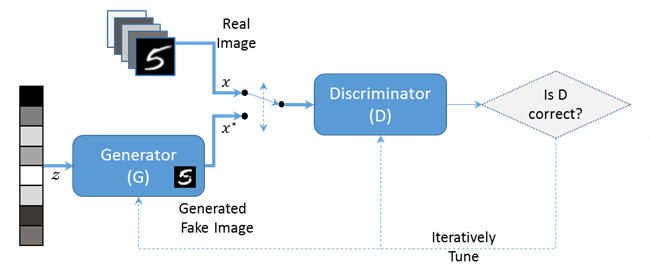
\includegraphics[width=0.9\textwidth]{figures/gan_model.png}
    \caption{GAN Structure}
    \label{fig:gan_model}
  \end{figure}
\end{frame}
%%%%%%%%%%%%%%%%%%%%%%%%%%%%%%%%%%%%%%%%%%%%%%%%%%%%%%%%%%%%%
\begin{frame}{GAN Structure}
  The standard formulation of GAN is given by
  \[
    \min_G\max_D V(G, D)
  \]
  The conventional form of $V(G, D)$ is given by
  \begin{equation}
    \label{eq:vgd}
    \E_{\bd{x}\sim q_{\mathrm{data}}}[\log D(\bd{x})]
    + \E_{\hat{\bd{x}} \sim p_{\mathrm{G}}}[\log(1-D(G(\hat{\bd{x}})))]
  \end{equation}
\end{frame}
%%%%%%%%%%%%%%%%%%%%%%%%%%%%%%%%%%%%%%%%%%%%%%%%%%%%%%%%%%%%%
\begin{frame}{Why Unstable?}
  For the conventional form of $V(G, D)$ \eqref{eq:vgd} and a fixed generator
  G, it is known that \cite{goodfellow2014generative}, the optimal discriminator
  is given by
  \[
    D^{\star}_G(\bd{x}) = 
    \frac{q_{\mathrm{data}}(\bd{x})}
    {q_{\mathrm{data}}(\bd{x}) + p_G(\bd{x})}.
  \]
  This gives
  \[
    \begin{split}
      D^{\star}_G(\bd{x}) &= \sigma(f^*(\bd{x})), \\
      \text{where } 
      f^*(\bd{x}) &= \log q_{\mathrm{data}}(\bd{x}) - \log p_G(\bd{x}) \\
      \implies \nabla_{\bd{x}}f^*(\bd{x}) &=
      \frac{1}{q_{\mathrm{data}}(\bd{x})}
      \nabla_{\bd{x}}q_{\mathrm{data}}(\bd{x})
      -
      \frac{1}{p_G(\bd{x})}\nabla_{\bd{x}}p_G(\bd{x}).
    \end{split}
  \]
  \alert{The derivate of $f^*(\bd{x})$ can be unbounded or even incomputable.}
\end{frame}
%%%%%%%%%%%%%%%%%%%%%%%%%%%%%%%%%%%%%%%%%%%%%%%%%%%%%%%%%%%%%
\begin{frame}{Method}
  Formulate the discriminator as follows:
  $$
  f(\bd{x}, \theta) = W^{L+1}
                 a_L(W^L(
                     a_{L-1}(W^{L-1}
                 (\dots a_1(W^1 \bd{x}) \dots))))
  $$ 
  \vspace{-15pt}
  \begin{itemize}
    \item $\bd{x}$: input of the network
    \item $\theta := \{W^1, \dots, W^L, W^{L+1}\}$: learning parameters set
    \item $a_l$: element-wise non-linear function
  \end{itemize}
  \pause
  The final output of the discriminator is given by
  \[
    D(\bd{x}, \theta) = \mathcal{A}(f(\bd{x}, \theta))
  \]
\end{frame}
%%%%%%%%%%%%%%%%%%%%%%%%%%%%%%%%%%%%%%%%%%%%%%%%%%%%%%%%%%%%%
\begin{frame}{Spectral Normalization}
  The spectral normalization controls the Lipschitz constant of the
  discriminator function $f$ by iterativelly constraining the spectral norm
  of each layer $g: \bd{h}_{in} \mapsto \bd{h}_{out}$.
  \begin{definition}
    The Lipschitz norm $\Vert f \Vert_{\mathrm{Lip}}$ of funtion
    $f$ is smallest  value $M$ such that
    \[
      \frac{\Vert f(\bd{x}) - f(\bd{x}') \Vert_2}
      {\Vert \bd{x} - \bd{x}'\Vert_2} \le M
    \]
    for any $\bd{x} \neq \bd{x}'$.
    \label{def: lip-norm}
  \end{definition}
\end{frame}
%%%%%%%%%%%%%%%%%%%%%%%%%%%%%%%%%%%%%%%%%%%%%%%%%%%%%%%%%%%%%
\begin{frame}{Spectral Normalization}
  \begin{definition}
    The spectral norm of a matrix $\mathbf{A}$ is defined by
    \[
      \sigma(\mathbf{A}):= \sup_{\bd{h}:\bd{h} \neq \zo}
      \frac{\Vert \mathbf{A}\bd{h} \Vert_2}{\Vert \bd{h} \Vert_2}
      = \sup_{ \lVert \bd{h} \rVert_2 \le 1} \lVert \mathbf{A}\bd{h} \rVert_2
    \]
    \label{def:spectral-norm}
  \end{definition}
  \begin{itemize}
    \item spectral norm is actually matrix 2-norm
    \item spectral norm is the max singular value of $\mathbf{A}$
  \end{itemize}
\end{frame}
%%%%%%%%%%%%%%%%%%%%%%%%%%%%%%%%%%%%%%%%%%%%%%%%%%%%%%%%%%%%%
\begin{frame}{Spectral Normalization}
  Therefore, for a linear layer $g(\bd{h}) = W\bd{h}$,
  \[
    \lVert g \rVert_{\mathrm{Lip}} = \sup_{\bd{h}} \sigma(\nabla g(\bd{h}))
    = \sup_{\bd{h}} \sigma(W) = \sigma(W)
  \]
  If $ \lVert a_l \rVert_{\mathrm{Lip}} = 1$
  \footnote{\eg, ReLU and leaky ReLU}, we can use the inequality
  \[
    \lVert g_1 \circ g_2 \rVert_{\mathrm{Lip}} \le 
    \lVert g_1 \rVert_{\mathrm{Lip}} \cdot
    \lVert g_2 \rVert_{\mathrm{Lip}}
  \]
  to get 
  \[
    \begin{aligned}
      &\lipnorm{f} &\le &\lipnorm{(\bd{h}_L \mapsto W^{L+1}\bd{h}_L)} \cdot
      \lipnorm{a_L} \cdot \\ 
      & ~ & ~ &\lipnorm{(\bd{h}_{L-1} \mapsto W^{L}\bd{h}_{L-1})} \cdots
      \lipnorm{a_1} \cdot
      \lipnorm{(\bd{h}_0 \mapsto W^{1}\bd{h}_0)} \\
      & ~ &= &\prod_{l=1}^{L+1} \lipnorm{(\bd{h}_{l-1} 
      \mapsto W^{l}\bd{h}_{l-1})} 
      = \prod_{l=1}^{L+1}\sigma(W^l).
    \end{aligned}
  \]
\end{frame}
%%%%%%%%%%%%%%%%%%%%%%%%%%%%%%%%%%%%%%%%%%%%%%%%%%%%%%%%%%%%%
\begin{frame}{Spectral Normalization}
  Normalize the spectral norm of the weight matrix $W$ such that 
  $\sigma(W) = 1$:
  \begin{equation}
    \label{eq:sn}
    \bar{W}_{\mathrm{SN}} := W/\sigma(W).
  \end{equation}
  If we normalize each $W^l$ using \eqref{eq:sn}, together with the fact 
  $\sigma(\bar{W}_{\mathrm{SN}}) = 1$, we see that 
  \alert{$\lipnorm{f}$ is bounded above by 1}.
\end{frame}
%%%%%%%%%%%%%%%%%%%%%%%%%%%%%%%%%%%%%%%%%%%%%%%%%%%%%%%%%%%%%
\begin{frame}{Power Iteration}
  How to compute the max singular value $\sigma(W)$?
\begin{itemize}
  \item SVD? -- computation inefficient
  \item Power iteration -- ok
\end{itemize}
\end{frame}
%%%%%%%%%%%%%%%%%%%%%%%%%%%%%%%%%%%%%%%%%%%%%%%%%%%%%%%%%%%%%
\begin{frame}{Power Iteration}
  Brief view of power method. Suppose $A \in \reals^{n \times n}$ is 
  diagonalizable, with eigenvalues ordered that
  \[
    |\lambda_1| \ge |\lambda_2| \ge \cdots \ge |\lambda_n|.
  \]
  Then we have $A = V\Lambda V^{-1}$ where $\Lambda = \diag(\lambda_1, \cdots,
  \lambda_n)$, now
  \[
    \begin{gathered}
      A^k = V \Lambda^k V^{-1} \\
      \implies A^k V = V\Lambda^{k}.
    \end{gathered}
  \]
  Randomly chose $\bd{x} = V \tilde{\bd{x}} \in \reals^n$ and consider
  \[
    \begin{split}
      A^k \bd{x} &= A^k V \tilde{\bd{x}} = V \Lambda^k \tilde{\bd{x}}
      = \sum_{j=1}^n \bd{v}_j \lambda_j^k \tilde{x}_j \\
      &= \lambda_1^k \sum_{j=1}^n \left( \frac{\lambda_j}{\lambda_1} \right)^k
      \tilde{x}_j \bd{v}_j 
      \to
      \lambda_1^k \tilde{x}_1 \bd{v}_1.
    \end{split}
  \]
\end{frame}
%%%%%%%%%%%%%%%%%%%%%%%%%%%%%%%%%%%%%%%%%%%%%%%%%%%%%%%%%%%%%
\begin{frame}{Power Iteration}
  If $|\lambda_1| > |\lambda_2|$, $A^k \bd{x} \to c\bd{v}_1$ for sufficient
  large $k$. This is the idea behind power iteration:
  \[
    \bd{x}^{(k+1)} = \frac{A \bd{x}^{(k)}}{ \lVert A \bd{x}^{(k)} \rVert}
    = \frac{A^k \bd{x}^{(0)}}{ \lVert A^k \bd{x}^{(0)} \rVert}.
  \]
  As $\bd{v}_1$ is the eigenvector corresponding to the max 
  eigenvalue, noting that $V$ is orthonormal, we have 
  $\bd{x}^{(k)} \to \bd{v}_1$. So the max eigen value of $A$ is given by
  \[
    \lambda_1 = \bd{v}_1^T A \bd{v}_1 = 
    \left(\bd{x}^{(k)}\right)^T \bd{x}^{(k+1)}. 
  \]
\end{frame}
%%%%%%%%%%%%%%%%%%%%%%%%%%%%%%%%%%%%%%%%%%%%%%%%%%%%%%%%%%%%%
\begin{frame}{Gradient Analysis}
  Recall that
  \[
    \bar{W}_{\mathrm{SN}} := W / \sigma(W).
  \]
  The gradient of the normalized weight matrix w.r.t. $W_{ij}$ is
  \begin{align}
    \frac{\partial \snmat}{\partial W_{ij}} &= 
    \frac{E_{ij}}{\sigma(W)} - 
    \frac{W}{\sigma^2(W)}\frac{\partial \sigma(W)}{\partial W_{ij}} \\
    &= \frac{E_{ij}}{\sigma(W)} -
    \frac{[\bd{u}_1 \bd{v}_1^T]_{ij}}{\sigma^2(W)}W \\
    &= \frac{1}{\sigma(W)} \left(E_{ij} - [\bd{u}_1 \bd{v}_1^T]_{ij}
    \snmat\right),
  \end{align}
  where $E_{ij}$ is the matrix whose $(i,j)$-th entry is 1 and zero otherwise,
  and $\bd{u}_1$ and $\bd{v}_1$ are respectively the first left and right
  singular vectors of $W$.
\end{frame}
%%%%%%%%%%%%%%%%%%%%%%%%%%%%%%%%%%%%%%%%%%%%%%%%%%%%%%%%%%%%%
\begin{frame}{Gradient Analysis}
  \only<1>{
  If $\bd{h}$ is the hidden layer to be transformed by $\snmat$, the derivative
  of the $V(G, D)$ calculated over the mini-batch w.r.t. $W$ of the
  discriminator $D$ is given by
  }
  \begin{align}
    \frac{\partial V(G, D)}{\partial W} &= \frac{1}{\sigma(W)}
    (\hat{E}[\bd{\delta h}^T] - (\hat{E}[\bd{\delta}^T \snmat \bd{h}])
    \bd{u}_1 \bd{v}_1^T) \\
    &= \frac{1}{\sigma(W)} (\hat{E}[\bd{\delta h}^T] - 
    \lambda \bd{u}_1 \bd{v}_1^T) \label{eq: ga}
  \end{align}
  \only<1>{
  \begin{itemize}
    \item $\bd{\delta} := (\partial V(G, D) / \partial(\snmat \bd{h}))^T$
    \item $\lambda := \hat{E}[\bd{\delta}^T(\snmat \bd{h})]$
    \item $\hat{E}[\cdot]$: empirical expectation over the mini-batch
  \end{itemize}
  }
  \only<2>{
  \begin{itemize}
    \item The first term $\hat{E}[\bd{\delta h}^T]$ of \eqref{eq: ga} is s
          ame as the derivative w/o spectral normalization
    \item The second term can be seen as a regularizer with adaptive
          coefficient $\lambda$
    \item $\lambda > 0$ if $\bd{\delta}$ and $\snmat \bd{h}$ point to same
          direction, thus gives a penalty
  \end{itemize}
  }
  \only<3>{
  \alert{Spectral normalization prevents the transformation of each layer 
  from being too sensitive in one direction.}
  }
\end{frame}
%%%%%%%%%%%%%%%%%%%%%%%%%%%%%%%%%%%%%%%%%%%%%%%%%%%%%%%%%%%%%
\section{Experiments}
\begin{frame}{Metrics}
  Assessment metrics:
  \begin{itemize}
    \item Inception Score (IS)\cite{salimans2016improved}: KL divergence 
          between conditional and marginal class distribution, higher is better
    \item Fréchet Inception Distance (FID)\cite{heusel2017gans}: Wassertein-2
          distance between generated and real images, lower is better
  \end{itemize}
\end{frame}
%%%%%%%%%%%%%%%%%%%%%%%%%%%%%%%%%%%%%%%%%%%%%%%%%%%%%%%%%%%%%
\begin{frame}{Experiments}
  The spectral norm of each layer in the discriminator dosen't change much
  in the course of training, they tends to be stablized.
  \begin{figure}[bp]
    \centering
    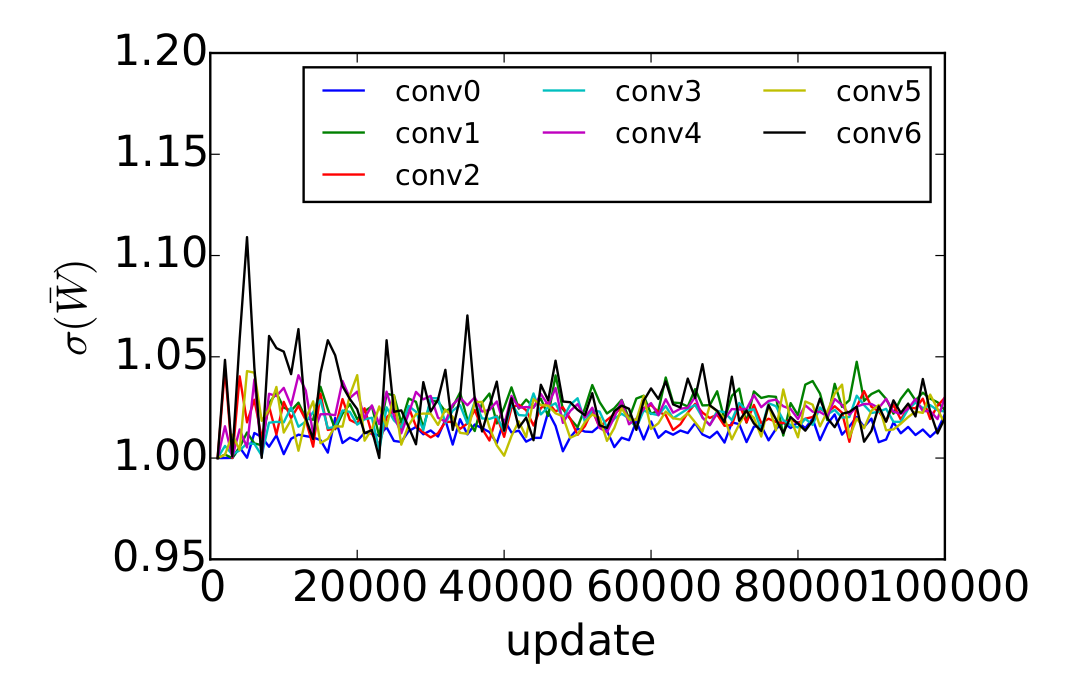
\includegraphics[width=0.7\textwidth]{figures/sn-change.png}
    \caption{Spectral norm changes during training}
    \label{fig:sn-change}
  \end{figure}
\end{frame}
%%%%%%%%%%%%%%%%%%%%%%%%%%%%%%%%%%%%%%%%%%%%%%%%%%%%%%%%%%%%%
\begin{frame}{Experiments}
  Spectral normalization is more robust than others w.r.t. different
  settings of hyperparameters.
  \begin{figure}[bp]
    \centering
    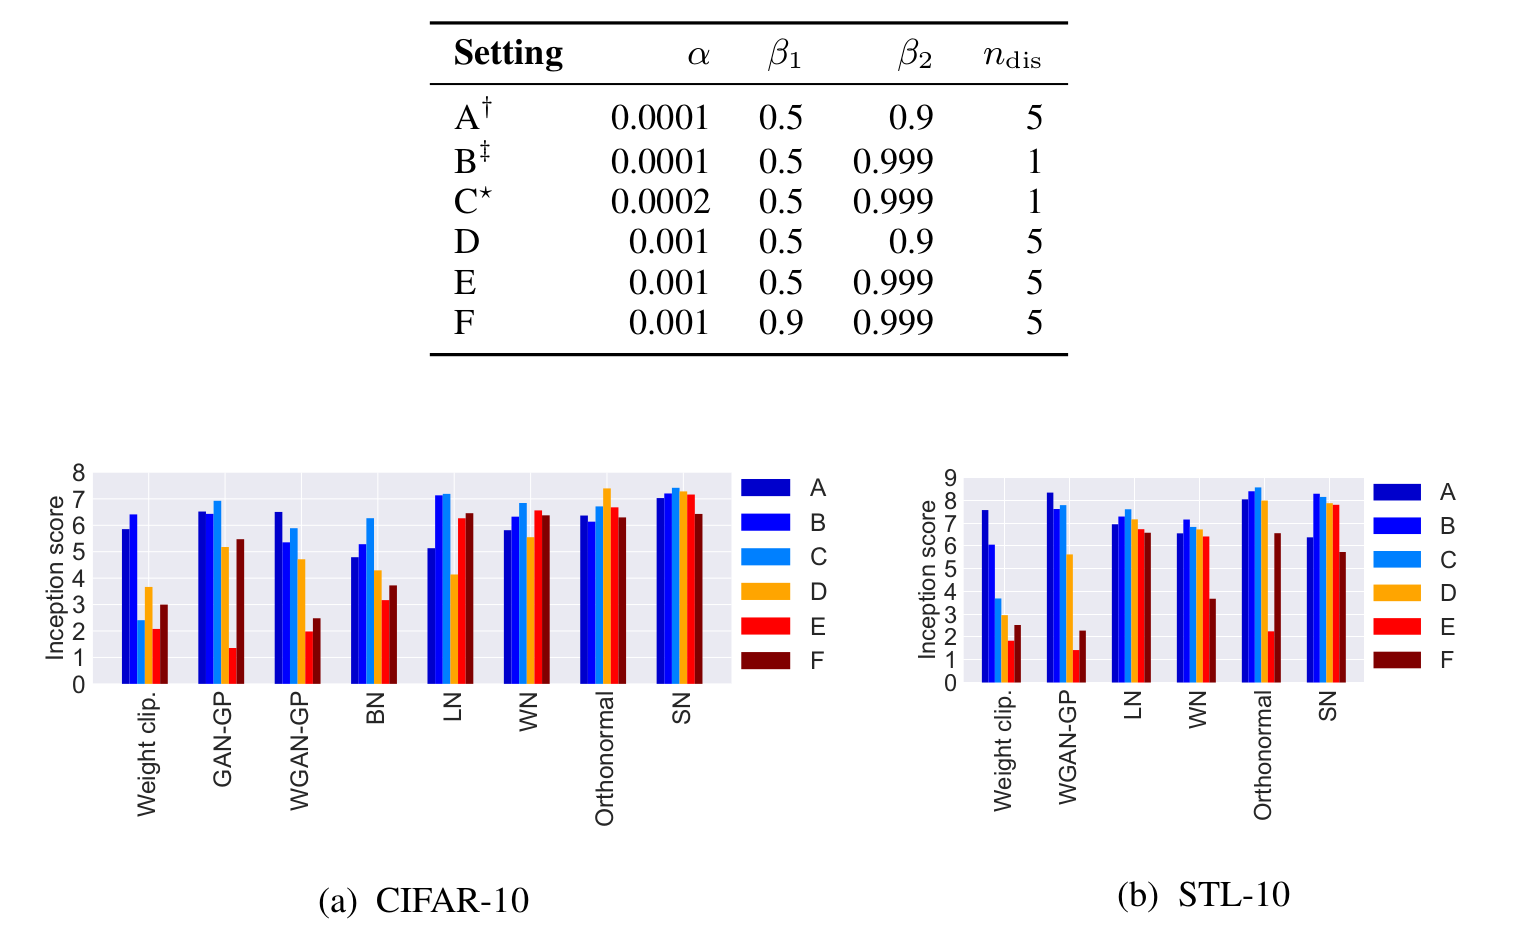
\includegraphics[width=0.9\textwidth]{figures/inception-score.png}
    \caption{Inception scores on CIFAR-10 and STL-10}
    \label{fig:is}
  \end{figure}
\end{frame}
%%%%%%%%%%%%%%%%%%%%%%%%%%%%%%%%%%%%%%%%%%%%%%%%%%%%%%%%%%%%%
\begin{frame}
  Spectral normalized GAN (SN-GAN) generates better images. (Hope you can
  see it.)
  \begin{figure}[bp]
    \centering
    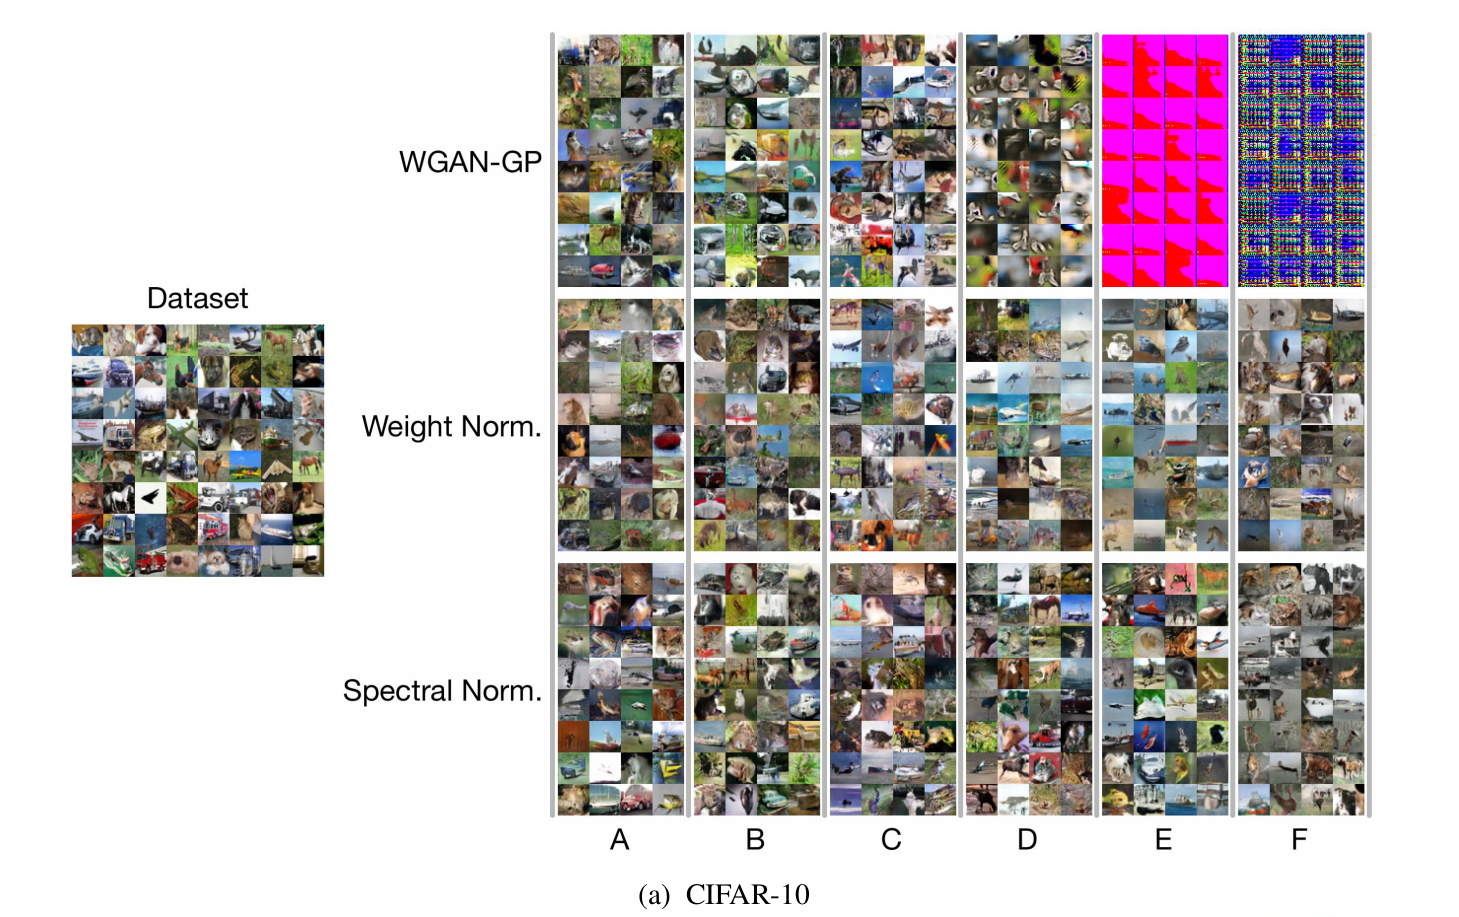
\includegraphics[width=0.9\textwidth]{figures/generated.png}
    \caption{Generated images on different methods on CIFAR-10}
    \label{fig:generated}
  \end{figure}
\end{frame}
%%%%%%%%%%%%%%%%%%%%%%%%%%%%%%%%%%%%%%%%%%%%%%%%%%%%%%%%%%%%%
\begin{frame}
  ILSVRC2012 dataset: large high dimensional.
  \begin{figure}[bp]
    \centering
    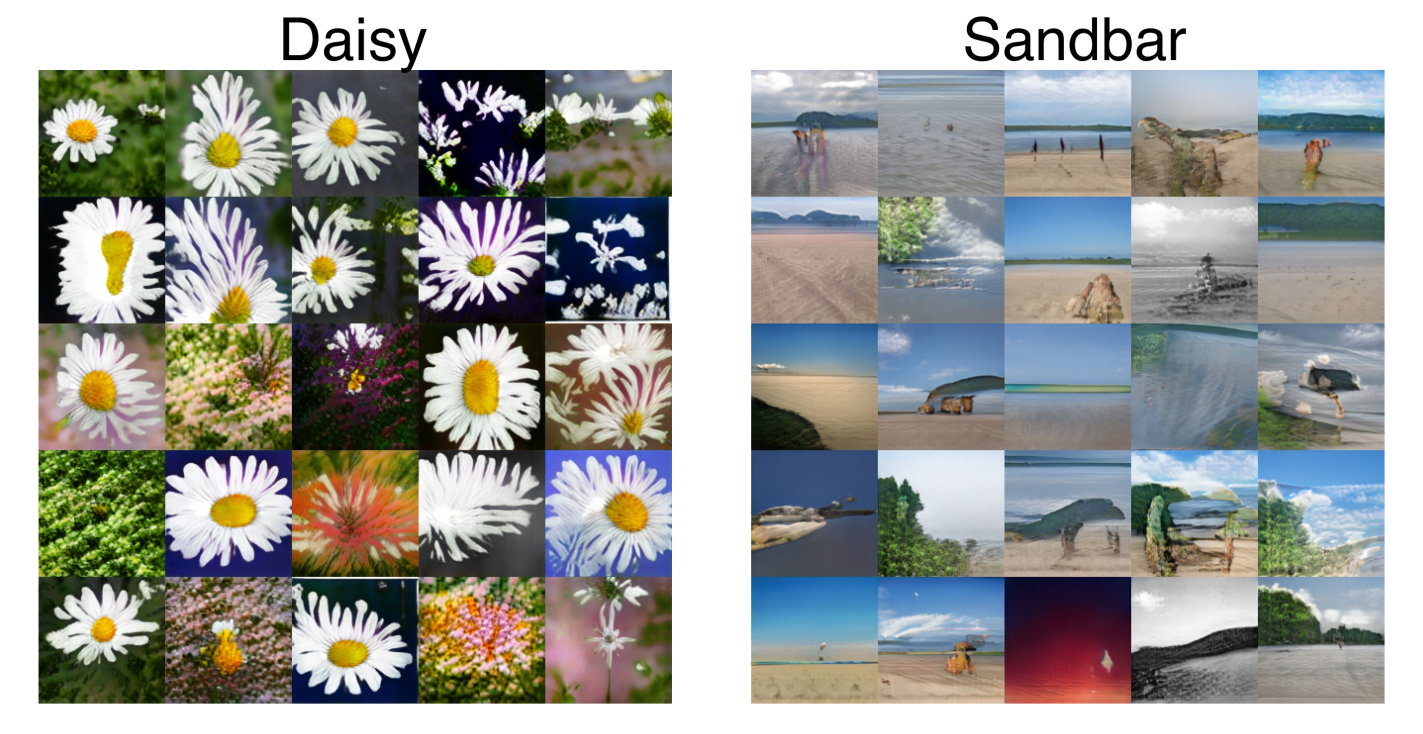
\includegraphics[width=0.9\textwidth]{figures/generated-ilsvr.png}
    \caption{128x128 pixel images generated by SN-GANs trained on ILSVRC2012
    dataset}
    \label{fig:generated-ilsvr}
  \end{figure}
\end{frame}
%%%%%%%%%%%%%%%%%%%%%%%%%%%%%%%%%%%%%%%%%%%%%%%%%%%%%%%%%%%%%
\begin{frame}{Singular Value Visualization}
  \only<1>{
  \begin{figure}[bp]
    \centering
    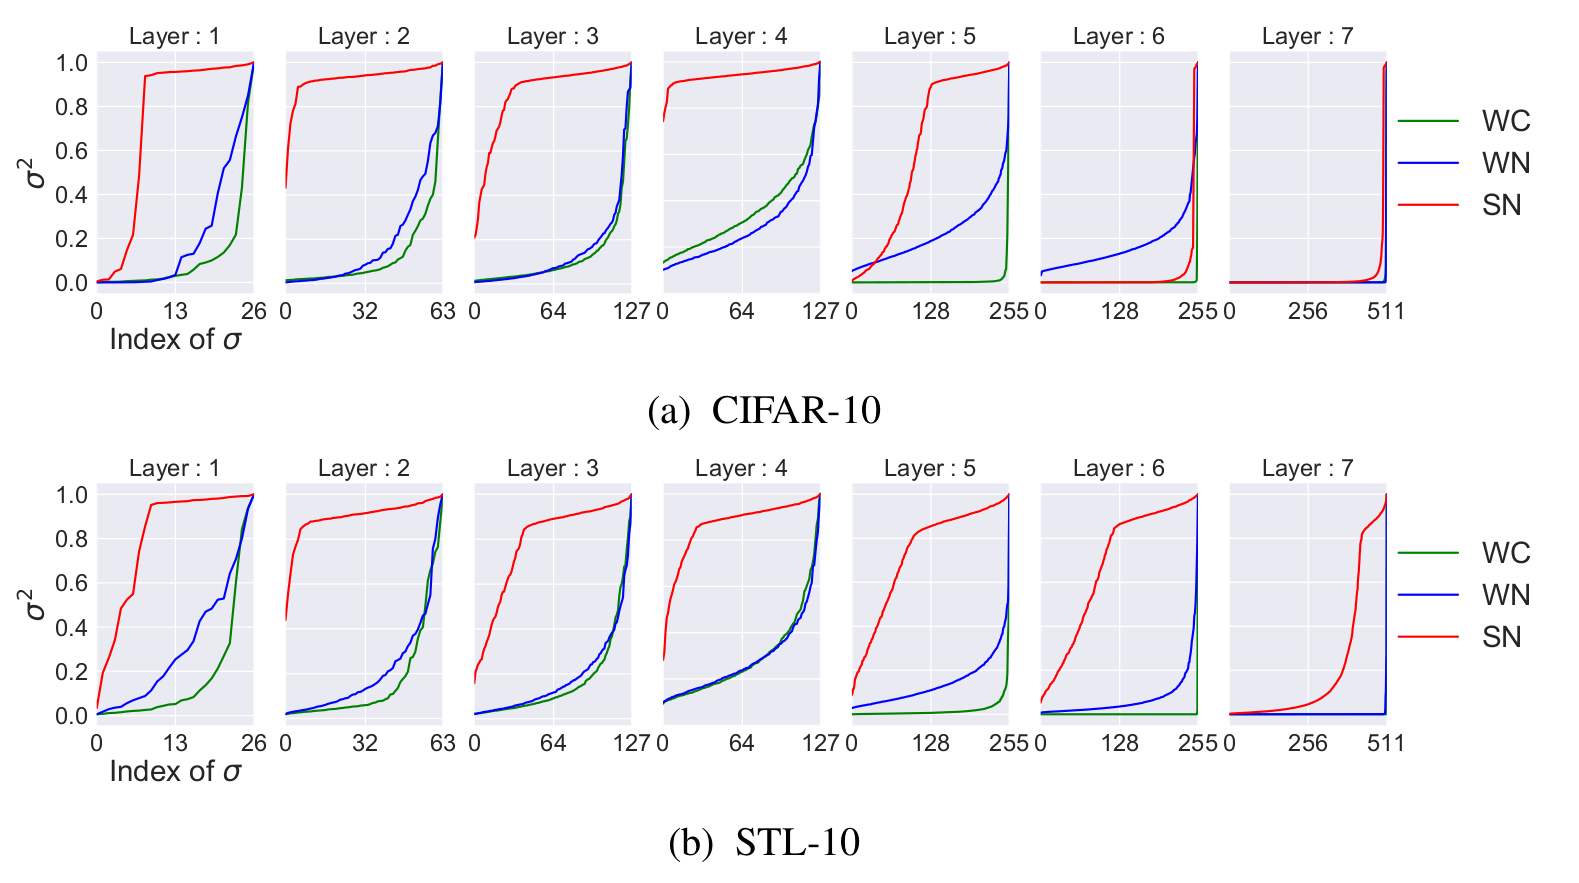
\includegraphics[width=0.9\textwidth]{figures/sv-visual.png}
    \caption{Squared singular value of weigth matrix trained with different
    methods: Weight Clipping (WC), Weight Normalization (WN), Spectral
    Normalization (SN)}
    \label{fig:sv-visual}
  \end{figure}
  }
  \only<2>{
    \begin{itemize}
      \item recall that SN can prevent the column space of weight matrix from
            being concentrating on one direction
      \item thus the singular values is more broadly distributed
      \item thus SN-GAN can generate more diversity, relatively
    \end{itemize}
  }
\end{frame}
%%%%%%%%%%%%%%%%%%%%%%%%%%%%%%%%%%%%%%%%%%%%%%%%%%%%%%%%%%%%%
\begin{frame}{Training Time}
  \begin{figure}[bp]
    \centering
    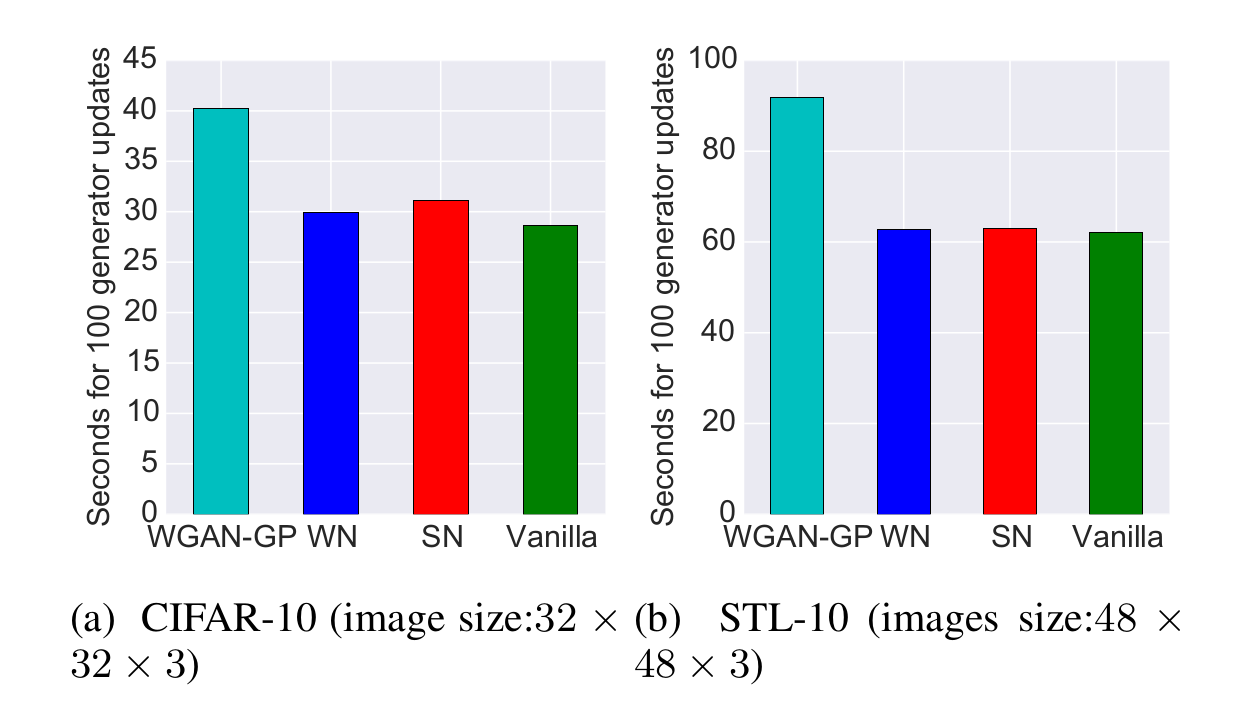
\includegraphics[width=0.8\textwidth]{figures/train-time.png}
    \caption{Computational time for 100 updates}
    \label{fig:train-time}
  \end{figure}
\end{frame}
%%%%%%%%%%%%%%%%%%%%%%%%%%%%%%%%%%%%%%%%%%%%%%%%%%%%%%%%%%%%%
\section{Conclusion}
\begin{frame}{Conclusion}
  \begin{itemize}
    \item Proposed spectral normalization as a stabilizer
    \item SN-GANs generate more diversity and have better performance
    \item Spectral normalization is computational light
  \end{itemize}
\end{frame}
%%%%%%%%%%%%%%%%%%%%%%%%%%%%%%%%%%%%%%%%%%%%%%%%%%%%%%%%%%%%%
\begin{frame}{References}
    \bibliographystyle{ieeetr}
    \bibliography{./spec.bib}
\end{frame}
%%%%%%%%%%%%%%%%%%%%%%%%%%%%%%%%%%%%%%%%%%%%%%%%%%%%%%%%%%%%%
\begin{frame}[standout]
    \Huge Thank you!
\end{frame}

% \begin{frame}[label=conclusion, standout]{Conclusion}
%   Awesome slide
% \end{frame}
\end{document}


